\insertmeeting 
	{Meet 1 Reflections} 
	{11-15-22} 
	{Odyssey Charter School}
	{Anouska, Jensen, Jorge, Karissa, Laura, Nathan, Ritam, Robert, Samantha, Tyler}
	{Images/RobotPics/robot.jpg}
	{2:30 - 4:30}
	
\hhscommittee{General}
\noindent\hfil\rule{\textwidth}{.4pt}\hfil
\subsubsection*{Goals}
\begin{itemize}
    \item Reflect on our first meet of the season at Odyssey Charter School
    \item Assess how to improve
    \item Analyze successes and sources of failure during matches
    \item Propose ideas on how to improve what we currently have

\end{itemize} 

\noindent\hfil\rule{\textwidth}{.4pt}\hfil

\subsubsection*{Accomplishments}
Walking into our first meet of the 2022-23 season, we had mixed feelings. Sure, our drive train was CADed, our vision worked great based on our testing, and we had an autonomous that at its best, will net us 21 points. We were missing one important asset though, an arm. Our locking mechanism intended to use on the extending poles was too weak to withstand the stress, which we only found out the night before. We couldn't lift any cones, and only had a quickly thrown together wooden funnel to compensate. If we were to rank well, we needed expert driving, good strategy, and a bit of luck to succeed.
For hardware, the only emergency was that during one of our matches, our servo broke, so we had to replace it, but we still earned enough points to win the match by then, and we got it fixed during the down time that followed. Our drive train did very well outside of that, it maneuvered around the poles without much trouble and can do so very speedily. Of course, that doesn't mean our hardware is perfect though, obviously we need to get our poles constructed in order to have a good robot. Going forward, we need to use a servo with a metal gear rather than a plastic one, as well as complete our pole design.
When it came to software, we had a major issue in that vision did not work as expected. It worked perfectly in testing, but under the different lighting of Oviedo High School's gym, the green would sometimes be read as a different color. We managed to fix it between our matches. In general, our autonomous was functional, and got us 21 points when it worked as intended. However, we only take about 15 seconds to complete it, and we can make what we have more efficient. By using more Roadrunner Algorithms, which allow us to make more smooth movements, we aim to create a more efficient autonomous more capable of doing more within autonomous. The Tele-Op did what it was designed to do, but it couldn't do much. With the limited space of the manual cone loading zone, we often had to agree to allow larger teams to hog the zone, or just got blocked by them in general. However, completing the pole design should help with this problem. We'll need to wait until we complete the pole design to see if there are any improvements to be made.
To detail the matches, we found that getting cones in the ground junctions are more difficult than expected. They are valuable obstacle for other robots. However, the corner goals are very easy and quick to score in, so as a ground based robot, we needed to decide between defense and scoring. Scoring ended up being the better option, since there's just so many more points that can be earned that way.
As for our overall performance, we managed to win four of our six matches, landing us 5th place overall, which isn't where we would like to be by League Championships, but for our circumstances, it is a solid outcome. Going forward, our goal for Meet 2 is to rise in rank, hopefully with a better auto and our poles constructed. Our overall long term goal is to rank as high as possible, but at a minimum in 4th place so we can participate in the finals during Leagues.
 

\begin{figure}[ht]
\centering
\begin{minipage}[b]{.48\textwidth}
  \centering
  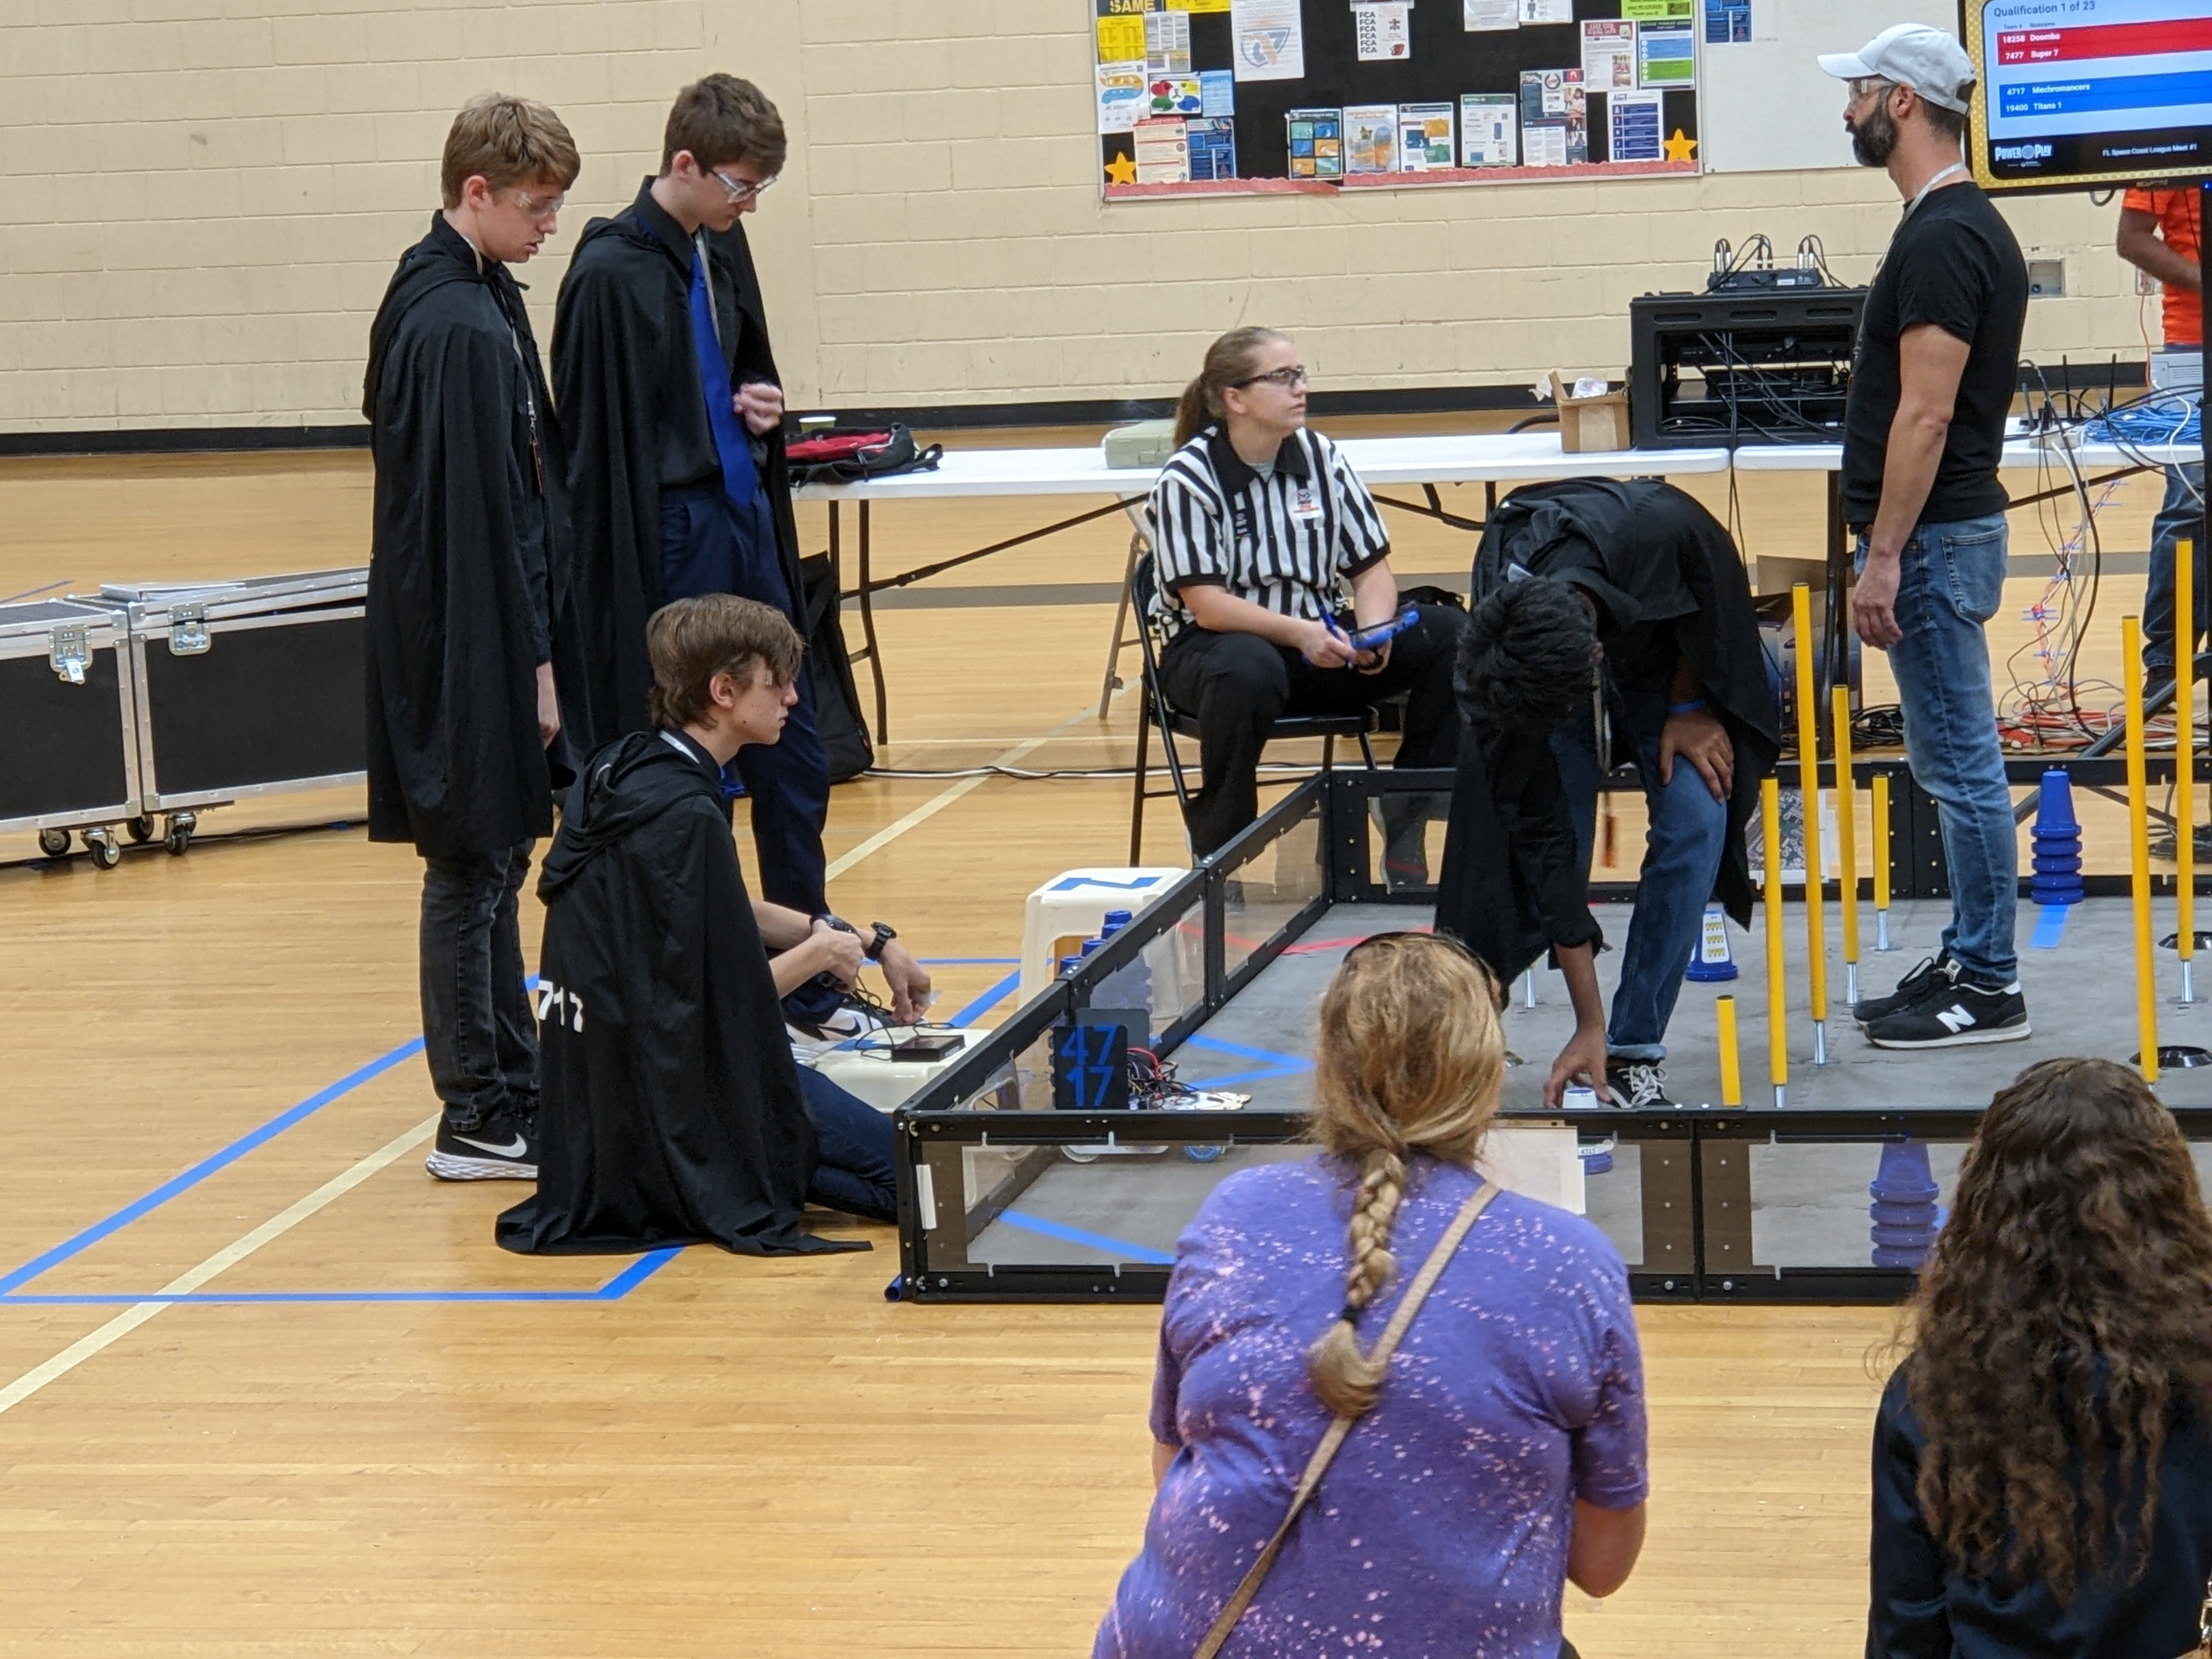
\includegraphics[width=0.95\textwidth]{Meetings/November/11-15-22/11-15-22-Field.jpg}
  \caption{Drive team on field}
  \label{fig:pic1}
\end{minipage}%
\hfill%
\begin{minipage}[b]{.48\textwidth}
  \centering
  \includegraphics[width=0.95\textwidth]{Meetings/November/11-15-22/11-15-22-Robot.JPG}
  \caption{Robot at first meet}
  \label{fig:pic2}
\end{minipage}
\end{figure}

\whatsnext{
\begin{itemize}
    \item Work on assembling poles 
    \item Propose new tele-op strategy
    
\end{itemize} 
}
